\documentclass[border=10pt]{standalone}
\usepackage{circuitikz}
\usepackage{tikz}
\usetikzlibrary{positioning, arrows.meta, calc}

\begin{document}

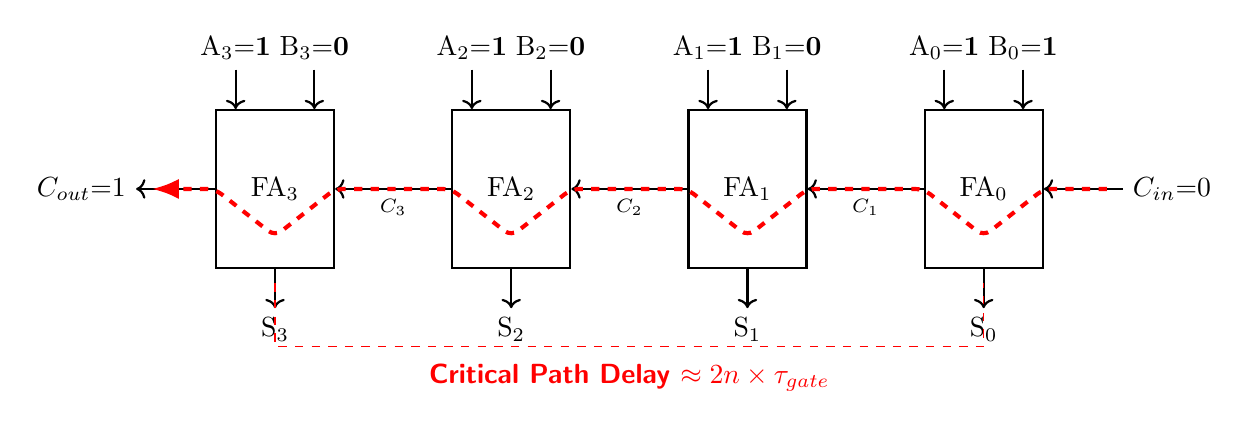
\begin{tikzpicture}[
    fa/.style={draw, thick, rectangle, minimum width=1.5cm, minimum height=2cm, fill=white},
    prop/.style={->, >=Latex, draw=red, line width=1.5pt,dashed},
    label/.style={font=\sffamily\small}
]

    % Full Adders (Right to Left: LSB to MSB)
    \node[fa] (fa0) at (0,0) {FA$_0$};
    \node[fa] (fa1) at (-3,0) {FA$_1$};
    \node[fa] (fa2) at (-6,0) {FA$_2$};
    \node[fa] (fa3) at (-9,0) {FA$_3$};

    % Inputs (A=1111, B=0001)
    \foreach \i/\a/\b in {0/1/1, 1/1/0, 2/1/0, 3/1/0} {
        \node[above=0.5cm of fa\i.north, xshift=-0.5cm,] (a\i) {A$_{\i}$=\textbf{\a}};
        \node[above=0.5cm of fa\i.north, xshift=0.5cm] (b\i) {B$_{\i}$=\textbf{\b}};
        \draw[thick, ->] (a\i.south) -- ([xshift=-0.5cm]fa\i.north);
        \draw[thick, ->] (b\i.south) -- ([xshift=0.5cm]fa\i.north);
        
        \node[below=0.5cm of fa\i.south] (s\i) {S$_{\i}$};
        \draw[thick, ->] (fa\i.south) -- (s\i.north);
    }
    
    % Carry Chain
    \draw[thick, ->] ([xshift=1cm]fa0.east) node[right]{$C_{in}$=0} -- (fa0.east);
    \draw[thick, ->] (fa0.west) -- (fa1.east) node[midway, below, font=\scriptsize] {$C_1$};
    \draw[thick, ->] (fa1.west) -- (fa2.east) node[midway, below, font=\scriptsize] {$C_2$};
    \draw[thick, ->] (fa2.west) -- (fa3.east) node[midway, below, font=\scriptsize] {$C_3$};
    \draw[thick, ->] (fa3.west) -- ([xshift=-1cm]fa3.west) node[left]{$C_{out}$=1};

    % Propagation Path (Red Zig-Zag or Straight line)
    % We want to visualize the flow FROM Cin to Cout passing through logic
    % Bending the line inside the FAs to avoid the text
    \draw[prop, rounded corners=3pt] 
        ([xshift=0.8cm]fa0.east) -- (fa0.east) -- ([yshift=-0.6cm]fa0.center) -- (fa0.west) -- 
        (fa1.east) -- ([yshift=-0.6cm]fa1.center) -- (fa1.west) -- 
        (fa2.east) -- ([yshift=-0.6cm]fa2.center) -- (fa2.west) -- 
        (fa3.east) -- ([yshift=-0.6cm]fa3.center) -- (fa3.west) -- 
        ([xshift=-0.8cm]fa3.west);

    % Delay Label
    \node[red, font=\bfseries\sffamily, align=center] at (-4.5, -2.4) {Critical Path Delay $\approx 2n \times \tau_{gate}$};
    \draw[red, dashed] (-9, -1.2) -- (-9, -2) -- (0, -2) -- (0, -1.2);

\end{tikzpicture}

\end{document}
